\documentclass[../main/Notas_de_aula.tex]{subfiles}

\begin{document}

\chapter{Construção de espaços de probabilidade}

Nessa seção descreveremos diversas maneiras diferentes de construir um espaço de probabilidade, dando diversos exemplos de como elas podem ser usadas na modelagem de diferentes processos reais.

\section{Caso enumerável}

Quando $\Omega$ é finito ou enumerável, tipicamente definimos sobre $\Omega$ a $\sigma$-álgebra das partes, ou seja $\mathcal{F} = \mathcal{P}(\Omega) = \sigma(\{\omega\}_{\omega \in \Omega})$.
Além disso podemos definir probabilidades sobre $(\Omega, \mathcal{F})$ de maneira simples tomando $(p_\omega)_{\omega \in \Omega}$ tais que
\begin{enumerate}[\quad a)]
\item $p_\omega \geq 0$ para todo $\omega \in \Omega$ e
\item $\sum_{\omega \in \Omega} p_\omega = 1$.
\end{enumerate}
De fato, nesse caso definimos $P(A) = \sum_{\omega \in A} p_\omega$ que claramente define uma probabilidade.

\begin{exercise}
  Mostre que se $\Omega$ é finito ou enumerável, toda probabilidade sobre $(\Omega, \mathcal{P}(\Omega))$ é dada como na descrição acima.
\end{exercise}

\begin{example} \mbox{}
  \begin{enumerate}[\quad a)]
  \item Dado $p \in [0,1]$, definimos a medida $\Ber(p)$ \index{distribuicao@distribuição!de Bernoulli} (em homenagem a Bernoulli) em $\{0,1\}$ com $p_1 = p, p_0 = 1-p$.
  \item Dados $n \geq 1$ e $p \in [0,1]$, definimos a medida $\Bin(n,p)$ \index{distribuicao@distribuição!binomial} (binomial) em $\Omega = \{0, 1, \dots, n\}$ com
    \begin{equation}
      p_i = \binom ni p^i (1-p)^{n-i}, \text{ para $i \in \Omega$.}
    \end{equation}
  \item Dado $p \in (0,1]$, em $\Omega = \{0, 1, \dots\}$ definimos a medida $\Geo(p)$ \index{distribuicao@distribuição!geometrica@geométrica} (geométrica) em $\Omega$ induzida pelos pesos
  \begin{equation}
    p_i = (1-p)^i p, \text{ para $i \geq 1$.}
  \end{equation}
  \end{enumerate}
\end{example}

\begin{exercise}
  Seja $\Omega = \{0,1\}^n$ e $p_\omega = \tfrac 1{2^n}$ para todo $\omega \in \Omega$ (ou seja a probabilidade uniforme).
  Considere $X: \Omega \to \{0,1, \dots, n\}$ dada por $X(\omega_1, \dots, \omega_n) = \sum_{i=1}^n \omega_i$.
  Obtenha a distribuição $P_X$.
  Dê um exemplo de medida em $\omega$ para a qual a distribuição de $X$ seja $\Bin(n,p)$.
\end{exercise}

\begin{topics}

\section{Tópico: Método Probabilístico}

Uma importante ferramenta em várias áreas da matemática, tais como Teoria dos Números, Combinatória e Teoria da Computação é o que chamamos de Método Probabilístico. \index{Metodo Probabilistico@Método Probabilístico}

Em várias situações, nós precisamos de mostrar a existência de objetos satisfazendo determinadas propriedades, mas não temos informação suficiente ou capacidade para construí-los explicitamente.
Nesse caso, podemos recorrer ao Método Probabilístico, que simplesmente nos sugere tomar um objeto aleatório de uma maneira esperta e mostrar que com probabilidade positiva as propriedades desejadas serão satisfeitas.
Esse método, apesar de muito ingênuo, é muito eficiente e em diversos casos provê os melhores exemplos conhecidos de certos objetos (para embaraço da comunidade científica).

Nessa seção daremos um exemplo em Teoria dos Números provido primeiramente por Erdõs\footnote{Somos gratos a Robert Morris por sugerir esse teorema como exemplo do Método Probabilístico.}.

\begin{theorem}[Erdös]
  Para todo conjunto finito $A \subset \mathbb{N}$, existe um sub-conjunto $B \subseteq A$ satisfazendo
  \begin{enumerate}[\quad a)]
  \item $\# B \geq \frac{\#A}{3}$ e tal que
  \item não existem $x, y$ e $z \in B$ com $x + y = z$.
  \end{enumerate}
  A propriedade $b)$ acima é o que chamamos de um conjunto ser livre de somas. \index{conjunto!livre de somas}
\end{theorem}

Certamente não temos muita informação sobre $A$, então vamos usar o método probabilístico para a prova desse teorema.

\begin{proof}
  Fixamos $p$ um número primo maior que três vezes o maior elemento de $A$ e considere o espaço $\mathbb{Z}_p$ dos inteiros módulo $p$.
  Seja $X$ um elemento aleatório de $\mathbb{Z}_p$ com distribuição uniforma, isto é $U_{\{0, \dots, p-1\}}$.
  \begin{exercise}
    Mostre que para todo $a \in A$, a multiplicação por $a$ é uma bijeção em $\mathbb{Z}_p$, ou seja
    \begin{equation}
      \mathbb{Z}_p \cdot a = \mathbb{Z}_p.
    \end{equation}
    onde o produto $\mathbb{Z}_p \cdot a$ é entendido elemento a elemento.
    Conclua que
    \begin{equation}
      P \Big[ X \cdot a \in \big[\tfrac p3, \tfrac {2p}3\big) \Big] \geq \frac 13 -\frac 1 p.
    \end{equation}
  \end{exercise}
  Definimos o conjunto aleatório
  $$\mathcal{B} = \{ x\in A \ | X\cdot a \in [\tfrac p3, \tfrac {2p}3) \},$$
  Esse conjunto e livre de soma: se $X=0$ o cojunto e vazio e nos outros casos se $x, y\in \mathcal{B}$
  $$(x+y)\in [\tfrac {2p}3, \tfrac {4p} 3)$$
  que e o complementario de $[\tfrac p3, \tfrac {2p}3)$ em $\mathbb{Z}_p$.

  \medskip

  Basta portanto mostrar que com probabilidade positiva $\# \mathcal{B} \geq \tfrac{\#A}3$, que segue do seguinte argumento.
  \begin{multline*}
    \int \# \mathcal{B} \d P = \int \sum_{a \in A} \1_{\big[ X \cdot a \in [p/3, 2p/3) \big]} \d P \\
    =
    \sum_{a \in A} P \Big[ X \cdot a \in \big[\tfrac p3, \tfrac {2p}3\big) \Big] \geq \frac{\# A}3- \frac{\# A} p> \frac{\# A-1 }3,
  \end{multline*}
  mas para qualquer variável aleatória ,  $P[X \geq \int X \d P] > 0$.
  Nesse caso, isso implica
  $P[X \ge \frac{\# A}3 ]=  P[X > \frac{\# A-1 }3 ]>0$.
\end{proof}

\todo{Adicionar contexto histórico: citar artigo Erdos e o Annals of Math que mostra que não é possível com $\#A(1/3 + \varepsilon)$.}

\end{topics}

\vfill
\pagebreak

\section{Caso absolutamente contínuo}

Uma outra maneira simples de definir um espaço de probabilidade, é partindo de um espaço de medida.
Seja $(\Omega, \mathcal{F}, \mu)$ um espaço de medida e $\rho:\Omega \to \mathbb{R}_+$ uma função mensurável com $\int \rho(x) \mu(\d x) = 1$.
Então podemos definir a probabilidade induzida
\begin{equation}
  \label{e:absolutamente_cont}
  P(A) = \int_A \rho(x) \mu(\d x).
\end{equation}
Nesse caso, chamamos $\rho$ de a \emph{densidade} \index{densidade} de $P$ com respeito a $\mu$.
Uma outra possível notação para a equação acima é $\d P = \rho(x) \d \mu$ \index{dP@$\d P = \rho \d \mu$} (lembrando a derivada de Radon-Nikodim).

Observe que o caso discreto pode ser definido em termos de uma densidade, onde $\rho(\omega) = p_\omega$ e $\mu$ é a medida da contagem em $\Omega$.

\begin{example}
  Vários exemplos podem ser obtidos via \eqref{e:absolutamente_cont} se tomamos $\Omega \subseteq \mathbb{R}$ e $\mu$ a medida de Lebesgue restrita a $\Omega$.
  Nesses casos, escrevemos $P = \rho(x) \d x$ em $\Omega$.
  Alguns exemplos importantes são:
  \begin{enumerate}[\quad a)]
  \item Para $a < b \in \mathbb{R}$, definimos a medida $U[a,b]$ \index{distribuicao@distribuição!uniforme} usando $\rho(x) = \tfrac{1}{b-a}\1_{[a,b]}(x)$.
  \item Para $\lambda > 0$, definimos a medida $\Exp(\lambda)$ \index{distribuicao@distribuição!exponencial} (chamada exponencial de parâmetro $\lambda$) por meio da densidade $\rho(x) = \lambda \exp\{-\lambda x\}$ em $[0,\infty)$.
  \end{enumerate}
\end{example}

Podemos também usar a distribuição de um elemento aleatório para construir outras probabilidades, como mostra o seguinte exemplo.

\begin{example}
  Considere por exemplo $X:[0,2\pi] \to \mathbb{C}$ dada por $X(t) = \exp\{-i t\}$.
  A distribuição imagem $X_*U_{[0,2\pi]}$ é o que chamamos de distribuição uniforme em $\mathbb{S}^1$, também denotada por $U_{S^1}$.
\end{example}

\begin{exercise}
  Mostre que $U_{\mathbb{S}^1}$ não é absolutamente contínua com respeito à medida de Lebesgue em $\mathbb{C} \sim \mathbb{R}^2$.
\end{exercise}

\begin{exercise}
  Mostre que $U_{\mathbb{S}^1}$ é invariante por rotações rígidas de $\mathbb{C}$, isto é, se $T:\mathbb{C} \to \mathbb{C}$ é uma isometria linear,
  $T_*U_{\mathbb{S}^1}=U_{\mathbb{S}^1}$.
\end{exercise}

\begin{exercise}
  Construa uma probabilidade em $S^2$ invariante por rotações.
\end{exercise}

\section{Funções acumuladas de distribuição}

Um caso muito importante de espaço amostral é $\Omega = \mathbb{R}$, principalmente por nos ajudar a entender distribuições de variáveis aleatórias.
Para tanto, precisaremos de uma boa ferramenta para descrever probabilidades em $\mathbb{R}$.

\begin{definition}
  Dada $P$ em $\mathbb{R}$, definimos $F_P:\mathbb{R} \to [0,1]$ por $F_P(x) = P\big((-\infty, x]\big)$.
  Essa função é chamada a \emph{função de distribuição} acumulada de $P$. \index{funcao de distribuicao@função de distribuição}
\end{definition}

\begin{notation}
  Se $X:\Omega \to \mathbb{R}$ é uma variável aleatória num espaço $(\Omega, \mathcal{F}, P)$, denotamos por $F_X$ \index{FX@$F_X$}
  a função de distribuição acumulada correspondente à distribuição $X_*P$.
\end{notation}

Lembramos que uma probabilidade em $\mathbb{R}$ é uma função $P:\mathcal{B}(\mathbb{R}) \to [0,1]$ e o domínio dessa função é bastante complicado.
Por exemplo se quisermos representar uma distribuição de uma variável aleatória no computador atravéz dessa função $P$, teríamos problemas.
Contudo, a função $F_P$ (ou $F_X$) é muito mais simples de ser compreendida ou representada, por seu domínio ser $\mathbb{R}$.

\begin{example}
  Não é difícil verificar que
  \begin{equation}
    F_{\delta_{x_0}} =
    \begin{cases}
      0 & \text{ se $x < x_0$,}\\
      1 & \text{ se $x \geq x_0$}
    \end{cases}
  \end{equation}
  e que
  \begin{equation}
    F_{U_{[0,1]}} =
    \begin{cases}
      0 & \text{ se $x \leq 0$,}\\
      x & \text{ se $x \in [0,1]$ e}\\
      1 & \text{ se $x \geq 1$.}
    \end{cases}
  \end{equation}
\end{example}

\begin{exercise}
  Calcule $F_{\Exp(\lambda)}$.
\end{exercise}

\begin{proposition}
  \label{p:propried_F}
  $F_P$ (e obviamente $F_X$) satisfazem:
  \begin{enumerate}[\quad a)]
  \item $\smash{\lim\limits_{x \to -\infty}} F(x) = 0$, $\smash{\lim\limits_{x \to \infty}} F(x) = 1$,
  \item $F$ é monótona não-decrescente e
  \item $F$ é contínua à direita e possui limite à esquerda (càdlàg, do francês). \index{cadlag@càdlàg}
  \end{enumerate}
\end{proposition}

\begin{proof}
  \begin{enumerate}[\quad a)]
  \item Se $x_n \to -\infty$ monotonamente, então $A_n = (-\infty, x_n]$ são encaixados e de interseção vazia.
    Logo, pela Proposição~\ref{p:prob_continua}, temos $P(A_n) \to 0$.
    O outro caso é análogo.
  \item Se $x \leq x'$ então $(-\infty, x] \subseteq (-\infty,x']$, donde $F(x) \leq F(x')$.
  \item Continuidade à direita (càd) - Se $x_n \downarrow x$ monotonamente, então $A_n = (-\infty, x_n] \downarrow (-\infty, x]$ (eles são encaixados).
    Logo $F(x_n) \to F(x)$.

    Limite à esquerda (làg) - Segue do fato de $F$ ser monótona e limitada. \qedhere
  \end{enumerate}
\end{proof}

\begin{theorem}
  \label{t:existe_prob_R}
  Se $F$ satisfaz as três propriedades listadas na Proposição~\ref{p:propried_F}, então existe uma única $P$ em $(\mathbb{R}, \mathcal{B}(\mathbb{R}))$ tal que $F = F_P$.
\end{theorem}

Poderíamos usar o Teorema da Extensão de Caratheodory para provar tal resultado, de maneira similar ao que foi feito no caso da Medida de Lebesgue.
Mas escolhemos abaixo um método mais simples, que parte da existência de $U_{[0,1]}$.

\begin{proof}
  A unicidade de tal $P$ segue da Proposição~\ref{p:P12_equal_pi} (consequêcia do Teorema de Dynkin), pois se $P$ e $P'$ são tais que $F_{P} = F_{P'}$, então temos que $P\big( (-\infty, x] \big) = P'\big( (-\infty, x] \big)$.
  Mas a classe de intervalos semi-infinitos da forma $(-\infty, x]$ forma um $\pi$-sistema que gera a $\sigma$-álgebra dos borelianos, logo $P = P'$.

  Para construir uma $P$ tal que $F_P = F$, definiremos $S:(0,1) \to \mathbb{R}$, a inversa generalizada de $F$, por
  \begin{equation}
    S(u) = \sup \{x \in \mathbb{R} \, : \,  F(x) < u\}.
  \end{equation}
  \begin{figure}[tb]
    \centering
    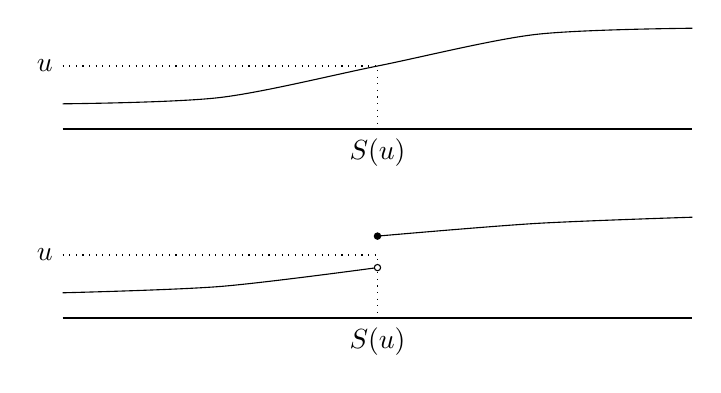
\begin{tikzpicture}[scale=.8]
      \draw (0,1) -- (10,1);
      \draw (0,4) -- (10,4); % second line
      \draw plot [smooth,tension=.5] coordinates{(0, 4.4) (2.5, 4.5) (5,5) (7.5, 5.5) (10, 5.6)};
      \draw plot [smooth,tension=.5] coordinates{(0, 1.4) (2.5, 1.5) (5,1.8)};
      \draw plot [smooth,tension=.5] coordinates{(5, 2.3) (7.5, 2.5) (10,2.6)};
      \draw[dotted] (0,5) -- (5,5) -- (5,4);
      \draw[dotted] (0,2) -- (5,2) -- (5,1);
      \draw [fill,color=white] (5,1.8) circle [radius=0.05];
      \draw (5,1.8) circle [radius=0.05];
      \draw [fill] (5,2.3) circle [radius=0.05];
      \node at (0,5) [left]{$u$};
      \node at (0,2) [left]{$u$};
      \node at (5,1) [below]{$S(u)$};
      \node at (5,4) [below]{$S(u)$};
    \end{tikzpicture}
    \caption{\small Ilustração da definição de $S(u)$.}
    \label{f:Rk_good}
  \end{figure}

  Seja $P = S_* U_{[0,1]}$, isto é $P(A) = U_{[0,1]}(S^{-1}(A))$ e mostraremos que $F_P = F$.
  Para tanto, basta ver que
  \begin{equation}
    \label{e:pseudo_inversa}
    \{u \in [0,1] \, : \,  S(u) \leq x\} = \{u \in [0,1] \, : \,  u \leq F(x)\}, \text{ para todo $x \in \mathbb{R}$}.
  \end{equation}
  Pois isso implicaria que $F_P(x) = U_{[0,1]}[S(u) \leq x] = U_{[0,1]} [u \leq F(x)] = F(x)$.

  Vamos agora checar \eqref{e:pseudo_inversa} observando que:
  \begin{enumerate}[\quad a)]
  \item Se $u \leq F(x)$ então todo $x'$ tal que $F(x') < u$ é menor que $x$.
    Logo $S(u) \leq x$.
  \item Por outro lado, se $x \ge S(u)$ então todo $x' > x$ satisfaz $F(x') > u$.
    Pois por continuidade a direita $F(x)\ge u$.
  \end{enumerate}
  Isos prova \eqref{e:pseudo_inversa}, terminando a prova da proposição.
\end{proof}

\begin{exercise}
  Mostre o resultado acima usando o Teorema de Extensão de Caratheodory.
\end{exercise}

\end{document}
